\chapter{Circuiti RC}

\renewcommand\thesection{\Roman{section}}

\section{Filtri RC}
\textbf{Obiettivo:} verificare il tipo di circuito, ricavare il rapporto di amplificazione del circuito e confrontare il valore della frequenza di taglio. 

\paragraph{Strumentazione:} 
\begin{enumerate}
    \item un alimentatore di tensione continua;
    \item una resistenza e un condensatore tali che la frequenza di taglio $f_0$ del circuito sia di qualche kHz;
    \item un voltmetro.
\end{enumerate}

\paragraph{Procedura:}
\begin{enumerate}
    \item costruire un circuito passa basso e un circuito passa alto scambiando la resistenza con il condensatore;
    \begin{figure}[h]
        \centering
        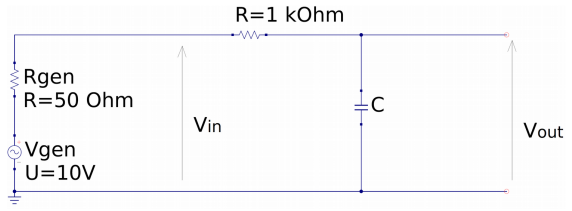
\includegraphics[width=0.6\linewidth]{Immagini/EXP3 - passabasso.png}
        \caption{filtro passa basso.}
        \label{fig: EXP3 - passabasso}
    \end{figure}
    \item misurare con l'oscilloscopio la tensione all'ingresso del circuito e all'uscita per varie frequenze;
    \item graficare il rapporto delle tensioni in funzione della frequenza;
    \item verificare che è un circuito passa alto o passa basso, effettuando una regressione;
    \item effettuare questa parte dell'analisi senza utilizzare le misure di R e C, ossia lavorando come se il quadrupolo fosse di costruzione incognita;
    \item confrontare il valore della frequenza di taglio ottenuta dalla regressione dei dati con il valore che si ottiene dalla misura di R e C. 
\end{enumerate}

\section{Derivatori ed integratori}

\textbf{Obiettivo:} verificare che i circuiti RC passa alto e passa basso sono funzionano anche come circuiti derivatori e integratori.

\paragraph{Procedura:}
nel caso di un passa alto l'equazione di maglia è $V_{in}=V_{out}+V_C$, dove 
\begin{equation}
    V_C=\frac{1}{C}\int idt+C,
\end{equation}
mentre ai capi della resistenza R si ha $V_{out}=Ri$, quindi l'equazione di maglia diventa
\begin{equation}
    V_{in}=V_{out}+\frac{1}{RC}\int V_{out}dt+C,
\end{equation}
dove se $V_{out}$ è trascurabile si ha
\begin{equation}
    V_{in}=\frac{1}{RC}\int V_{out}dt+C,
\end{equation}
la quale derivata restituisce
\begin{equation}
    V_{out}=RC\frac{dV_{in}}{dt}.
\end{equation}
La condizione necessaria è che $V_{out}$ sia trascurabile. Questa condizione si può ottenere se la costante di tempo RC è molto piccola rispetto al periodo della funzione d'onda in ingresso.
\begin{enumerate}
    \item Calcolare e poi verificare sperimentalmente il valore di R necessario per avere, alla frequenza di 1 kHz uno sfasamento fra tensione di ingresso ed uscita vicino a 90°;
    \item applicando delle onde quadre all'ingresso del circuito verificare sotto quali condizioni il circuito effettua la funzione di derivata;
    \item provare ad inviare un'onda triangolare ed osservare la tensione in uscita. 
\end{enumerate}
Nel caso di un passa basso l'equazione di maglia è $V_{in}=V_R+V_C=Ri+V_{out}$, ma derivando l'equazione di $V_C$ e sostituendola in questa equazione si ha
\begin{equation}
    V_{in}=RC\frac{dV_{out}}{dt}+V_{out}.
\end{equation}
Ipotizzando di poter trascurare $V_{out}$ ed integrando si ottiene
\begin{equation}
    V_{out}=\frac{1}{RC}\int V_{in}dt+C.
\end{equation}
La condizione per cui $V_{out}$ è trascurabile si può ottenere usando una costante di tempo RC grande rispetto al periodo della funzione d'onda in ingresso.
\begin{enumerate}
    \item Verificare sperimentalmente che, inviando con il generatore di funzioni un'onda quadra, si può ottenere l'integrale della tensione di ingresso. Si dovrebbe ottenere un'onda triangolare.
    \item Provare ad inviare un'onda triangolare e osservare la tensione in uscita.
\end{enumerate}

\setcounter{section}{0}
\renewcommand\thesection{\Alph{section}}

\section{Guadagno di un filtro RC}
Un circuito RC è un quadripolo composto da due elementi passivi (detti anche bipoli): una resistenza che ha un comportamento costante con il variare della frequenza; ed un condensatore la cui impedenza varia con l'inverso della frequenza. Usando il calcolo simbolico (applicabile solo se il segnale di ingresso è sinusoidale) si ha
\begin{equation}
    I = \frac{V_{in}}{R + (j\omega C)^{-1}}.
\end{equation}
Quindi, per il passa alto\footnote{Per il passa basso invece si ha $V_{out}=I/(j\omega C)$.}, si ha
\begin{equation}
 V_{out} = IR = \frac{V_{in}}{R + (j\omega C)^{-1}} R = \frac{V_{in}}{1 + (j\omega RC)^{-1}},
\end{equation}
facendone il modulo si ha 
\begin{equation}
    \left| V_{out} \right| = \frac{\left| V_{in} \right|}{\sqrt{1 + (\omega^2 R^2 C^2)^{-2}}}.
    \label{eq:placeholder}
\end{equation}
Sostituendo $RC=1/(2\pi f_0)$ si ottiene
\begin{equation}
A_V=\left| \frac{V_{out}}{V_{in}} \right| = \frac{1}{\sqrt{1 + f_0^2/f^2}} = \frac{f}{\sqrt{f^2 + f_0^2}},
\end{equation}
dove $A_V$ è il guadagno del quadripolo. \'E utile definire una frequenza limite. La convenzione è la frequenza $f = f_0$, dove il guadagno $A_V$ si riduce a
\begin{equation}
    |A_{VL}|=\frac{1}{\sqrt{2}},
\end{equation}
dove il pedice ``L'' sta per ``low'' cioè la minima frequenza che passa. La fase tra la tensione in uscita e quella in ingresso si ottiene da
\begin{equation}
\frac{V_{out}}{V_ {in}} = \frac{1}{1 + (\omega^2 R^2 C^2)^{-1}}\left(1 + \frac{j}{\omega RC}\right)\Rightarrow\tan{\phi}=\frac{1}{\omega RC}.
\end{equation}
Sostituendo $f_0$ si ha $\tan{\phi}=f_0/f$ e se $f=f_0$ si ha $\tan{\phi}=1\Rightarrow\phi=45$°.
Riassumendo:
\begin{itemize}
    \item per frequenze minori di $f_0$ il segnale di ingresso per convenzione non passa in uscita;
    \item per $f = f_0$ il segnale di uscita è $\sqrt{2}$ volte minore del segnale di ingresso e la tensione di uscita è di 45° in anticipo rispetto a quella di ingresso.
\end{itemize}
